\section{Introduzione}

Nim Multiplayer è un'applicazione web che permette a 2 o più utenti di giocare a Nim (\href{https://it.wikipedia.org/wiki/Nim}{https://it.wikipedia.org/wiki/Nim}). Nim è un gioco matematico che coinvolge 2 giocatori. Nim Multiplayer supporta le partite 1 vs 1, ed aggiunge regole per gestire le partite multi giocatore.

\begin{figure}[h]
	\centering
	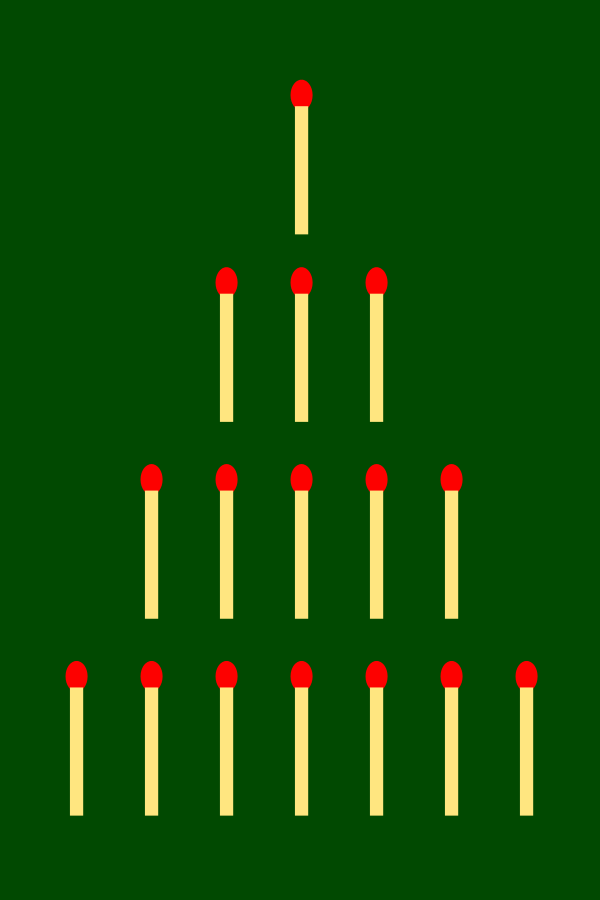
\includegraphics
	[width=0.25\linewidth]
	{wikipedia - 600px-NimGame.svg}
	\caption{una partita Nim\cite{nim_wikipedia}.}
	%\label{fig:nim-logo}
\end{figure}

Per giocare a Nim, i 2 giocatori, a turno, rimuovono gli "\emph{oggetti} o \emph{elementi}" da "\emph{cumuli} o \emph{pile}" distinti.

Per maggiore chiarezza, in questo progetto si è scelto di utilizzare termini più specifici (e ritenuti più appropriati) per esprimere il gergo del gioco: gli "\emph{oggetti} o \emph{elementi}", data la loro forma, assumono il nome di \emph{bastoncini}; mentre i "\emph{cumuli} o \emph{pile}" vengono definiti semplicemente come \emph{righe} o \emph{righe di bastoncini}.

Durante il proprio turno, la mossa consiste nel rimuovere un numero qualsiasi di bastoncini posti su una qualsiasi e unica riga, ma tali bastoncini devono essere adiacenti e tra loro non vi devono essere altri bastoncini già rimossi (non è possibile saltare la mossa nel proprio turno).

A seconda della versione, l'obiettivo del gioco è evitare di rimuovere l'ultimo bastoncino (versione \emph{Marienbad} o \emph{misère}) o rimuovere l'ultimo bastoncino (versione \emph{standard}).

Il numero di bastoncini e di righe sono concordati a piacere tra i giocatori all'inizio della partita.

Il Nim è divenuto piuttosto famoso perché ha una strategia di vittoria semplice (ha classe di complessità L), facilmente utilizzabile come esempio in teoria dei giochi, in particolare questa si basa sul calcolo binario\cite{nim_wikipedia}.

In breve, Nim Multiplayer modella: il gioco Nim tradizionale con vittoria \emph{standard} e \emph{Marienbad}; aggiunge una variante riguardo la rotazione dei turni (turni chaos); aggiunge regole per la gestione della vittoria \emph{standard} e \emph{Marienbad} in partite multi giocatore.

\newpage
